\documentclass{standalone}
\usepackage{tikz}
\begin{document}
    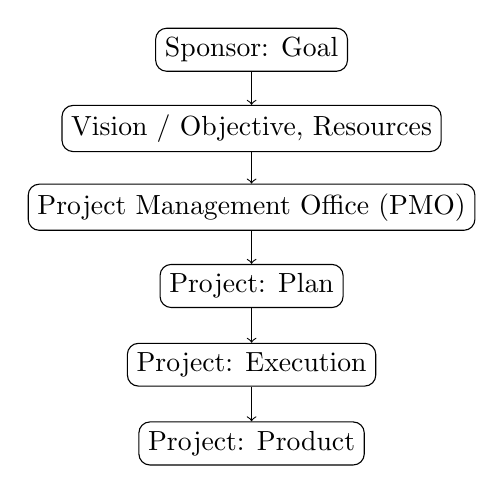
\begin{tikzpicture}[every node/.style={rounded corners}]
        \node[draw] (sp) at (0,0) {Sponsor: Goal};
        \node[draw, below of=sp] (vi) {Vision / Objective, Resources};
        \node[draw, below of=vi] (pmo) {Project Management Office (PMO)};
        \node[draw, below of=pmo] (pl)  {Project: Plan};
        \node[draw, below of=pl] (ex)  {Project: Execution};
        \node[draw, below of=ex] (pr)  {Project: Product};
        \draw[->] (sp) -- (vi);
        \draw[->] (vi) -- (pmo);
        \draw[->] (pmo) -- (pl);
        \draw[->] (pl) -- (ex);
        \draw[->] (ex) -- (pr);
    \end{tikzpicture}
\end{document}
